%
% management.tex
%
% Copyright (C) 2022 by SpaceLab.
%
% Camera Payload Preliminary Design Review
%
% This work is licensed under the Creative Commons Attribution-ShareAlike 4.0
% International License. To view a copy of this license,
% visit http://creativecommons.org/licenses/by-sa/4.0/.
%

%
% \brief Project management slides.
%
% \author Gabriel Mariano Marcelino <gabriel.mm8@gmail.com>
% \author Vitória Beatriz Bianchin <vitoriabbianchin@gmail.com>
% \author Caique Sales de Miranda Gomes <kiqsmg@gmail.com>
%
% \version 0.1.0
%
% \date 2022/06/24
%


\begin{frame}{Project Management}

    \begin{itemize}
        \item Activities and tasks: GitHub issues/project
        \vspace{0.25cm}
        \item Periodic meetings
        \vspace{0.25cm}
        \item Source files and versioning control: Git/GitHub repository (\href{https://github.com/spacelab-ufsc/camera}{\textcolor{blue}{https://github.com/spacelab-ufsc/slcam}}) with five development branches:
            \begin{itemize}
                \item \textit{dev\_doc}: Documentation
                \item \textit{dev\_hardware}: Hardware project
                \item \textit{dev\_firmware}: Firmware project
                \item \textit{dev\_software}: Software project
                \item \textit{dev\_mechanical}: Mechanical project
            \end{itemize}
    \end{itemize}

\end{frame}

% #########################################################################
% #########################################################################

\begin{frame}{Product Tree}

    \begin{figure}[!ht]
        \begin{center}
            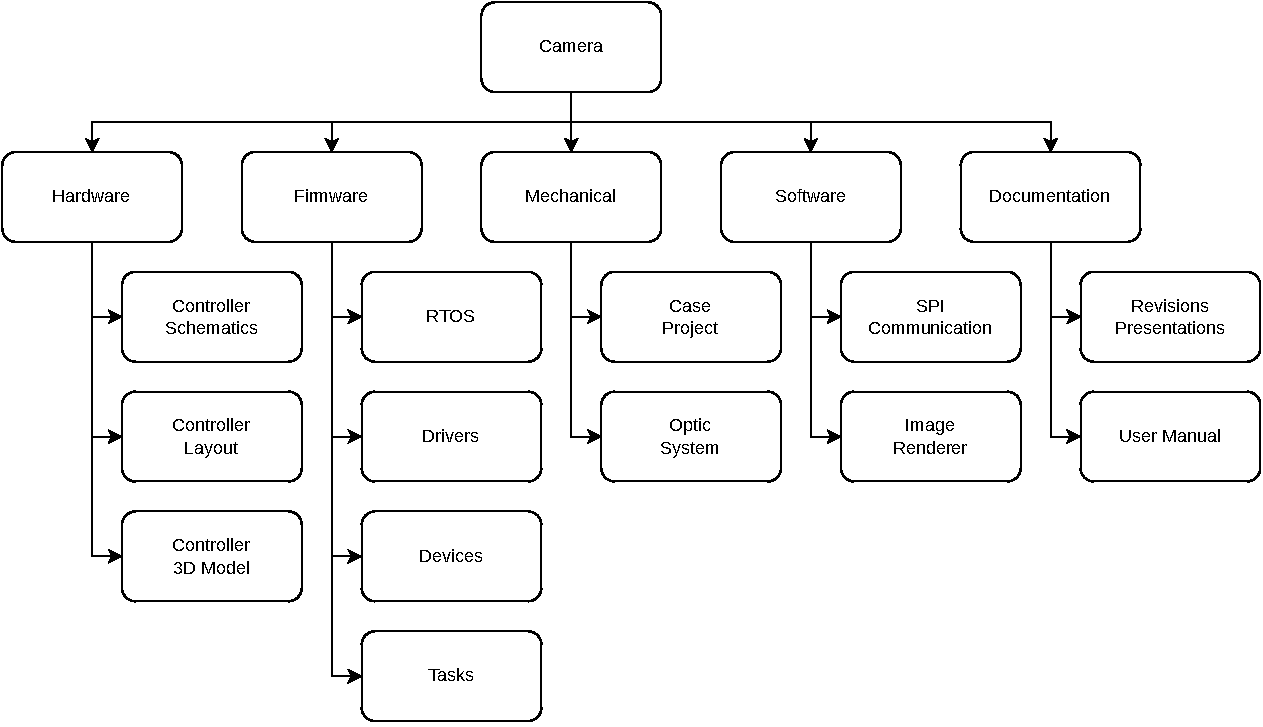
\includegraphics[width=11cm]{figures/product-tree-cam}
        \end{center}
    \end{figure}

\end{frame}

% #########################################################################
% #########################################################################

\begin{frame}{Schedule}

\begin{table}[!htb]\tiny
    \centering
    \label{tab:schedule}
    \begin{tabular}{lC{0.15cm}C{0.15cm}C{0.15cm}C{0.15cm}C{0.15cm}C{0.15cm}C{0.15cm}C{0.15cm}C{0.15cm}C{0.15cm}C{0.15cm}C{0.15cm}C{0.15cm}C{0.15cm}}
        \toprule[1.5pt]
        \multirow{2}{*}{\textbf{Activity}} & \multicolumn{13}{c}{\textbf{Week}} \\
                          & W0 & W1 & W2 & W3 & W4 & W5 & W6 & W7 & W8 & W9 & W10 & W11 & W12 & W13\\
        \midrule
        Project definition            & X &   &   &   &   &   &   &   &   &   &   &   &   &   \\
        Components aquisiton          & X & X & X & X &   &   &   &   &   &   &   &   &   &   \\
        Controller schematics         &   &   & X & X & X &   &   &   &   &   &   &   &   &   \\
        Mechanical structure design   &   &   & X & X & X & X &   &   &   &   &   &   &   &   \\
        \textbf{PDR}                  &   &   &   &   & X &   &   &   &   &   &   &   &   &   \\
        Controller PCB layout         &   &   &   &   &   & X & X & X &   &   &   &   &   &   \\
        Firmware development          &   &   &   &   &   & X & X & X & X & X & X & X &   &   \\
        Test software development     &   &   &   &   &   & X & X & X & X & X & X & X &   &   \\
        Mockup fabrication            &   &   &   &   &   &   &   & X &   &   &   &   &   &   \\
        \textbf{CDR}                  &   &   &   &   &   &   &   &   & X &   &   &   &   &   \\
        Controller PCB fabrication    &   &   &   &   &   &   &   &   & X & X & X & X &   &   \\
        Case fabrication              &   &   &   &   &   &   &   &   & X & X & X & X &   &   \\
        Electrical and firmware tests &   &   &   &   &   &   &   &   &   &   &   &   & X &   \\
        Mechanical integration        &   &   &   &   &   &   &   &   &   &   &   &   & X &   \\
        User manual preparation       &   &   &   &   &   &   &   &   &   &   & X & X & X &   \\
        \textbf{AR}                   &   &   &   &   &   &   &   &   &   &   &   &   &   & X \\
        \bottomrule[1.5pt]
    \end{tabular}
\end{table}

\end{frame}

% #########################################################################
% #########################################################################

\begin{frame}{Team}

\begin{table}[!htb]
    \centering
    \label{tab:team}
    \begin{tabular}{ll}
        \toprule[1.5pt]
        \textbf{Role} & \textbf{Name} \\
        \midrule
        Management/Support                    & Gabriel Mariano Marcelino \\
        Hardware design                       & Vitória Beatriz Bianchin \\
        \multirow{2}{*}{Firmware development} & \textcolor{red}{TBD} \\
                                              & Vitória Beatriz Bianchin \\
        Software development                  & \textcolor{red}{TBD} \\
        Mechanical design                     & Caique Sales de Miranda Gomes \\
        \bottomrule[1.5pt]
    \end{tabular}
\end{table}

\end{frame}

% #########################################################################
% #########################################################################

\begin{frame}{Cost Estimation\footnote{2 units.}}

\begin{table}[!htb]\scriptsize
    \centering
    \label{tab:cost-estimation}
    \begin{tabular}{lccc}
        \toprule[1.5pt]
        \textbf{Item} & \textbf{Unit (US\$)} & \textbf{Quantity} & \textbf{Total (US\$)} \\
        \midrule
        Arducam Mini 2MP Plus & 25,99 & 2  & 51,98 \\
        Lens                  & 7,99 \textcolor{red}{TBC} & 2  & 15,98 \\
        STM32 dev kit         & 2,50  & 2  & 5,00 \\
        STM32F103C8T6         & 7,31  & 2  & 14,62 \\
        W25Q128JVSIM          & 1,95  & 2  & 3,90 \\
        TPS2010AD             & 2,96  & 2  & 5,92 \\
        TCAN330GD             & 3,89  & 2  & 7,78 \\
        532610671             & 0,81  & 2  & 1,62 \\
        532610371             & 0,76  & 4  & 3,04 \\
        ECS-80-10-33-CHN-TR3  & 0,69  & 2  & 1,38 \\
        Passive components    & 2,00  & 1  & 2,00 \\
        PCB                   & 0,20  & 10 & 2,00 \\
        Case                  & 30 \textcolor{red}{TBC} & 2  & 60 \\
        \midrule
        Total          & \multicolumn{3}{c}{US\$175,92\footnote{Prices in June 2022, without delivery rates or taxes.}} \\
        \bottomrule[1.5pt]
    \end{tabular}
\end{table}

\end{frame}